\chapter{От малых городов до городов-миллионеров}
\label{ch:city}

Глава посвящена исследованию различных типов городов, соответствующих четырем объектам Викиданных — <<Малый город>>, <<Город>>, <<Большой город>> и <<Города-миллионеры>>. В ходе исследования с использованием SPARQL-запросов получены данные о количестве экземпляров исследуемых объектов, а также рассмотрены вопросы, связанные со свойствами population (численность населения) и sister city (город-побратим) этих объектов Викиданных. В том числе решены следующие задачи: подсчет и анализ численности населения разных типов городов; определение числа городов, не имеющих побратимов; построение списка городов, упорядоченного по числу побратимов; нахождение числа городов с определённым числом побратимов; определение страны с наибольшим числом побратимов; нахождение ближайших соседей России. В заключении работы дана оценка полноты данных, представленных в Википедии и Викиданных, и перечислены проблемы и сложности, возникшие при изучении объектов разных типов городов.

\section{Города-побратимы}
\subsection{Число городов с определенным числом побратимов}
\begin{marginfigure}[0.0cm]
{
\setlength{\fboxsep}{0pt}%
\setlength{\fboxrule}{1pt}%
\fcolorbox{gray}{gray}{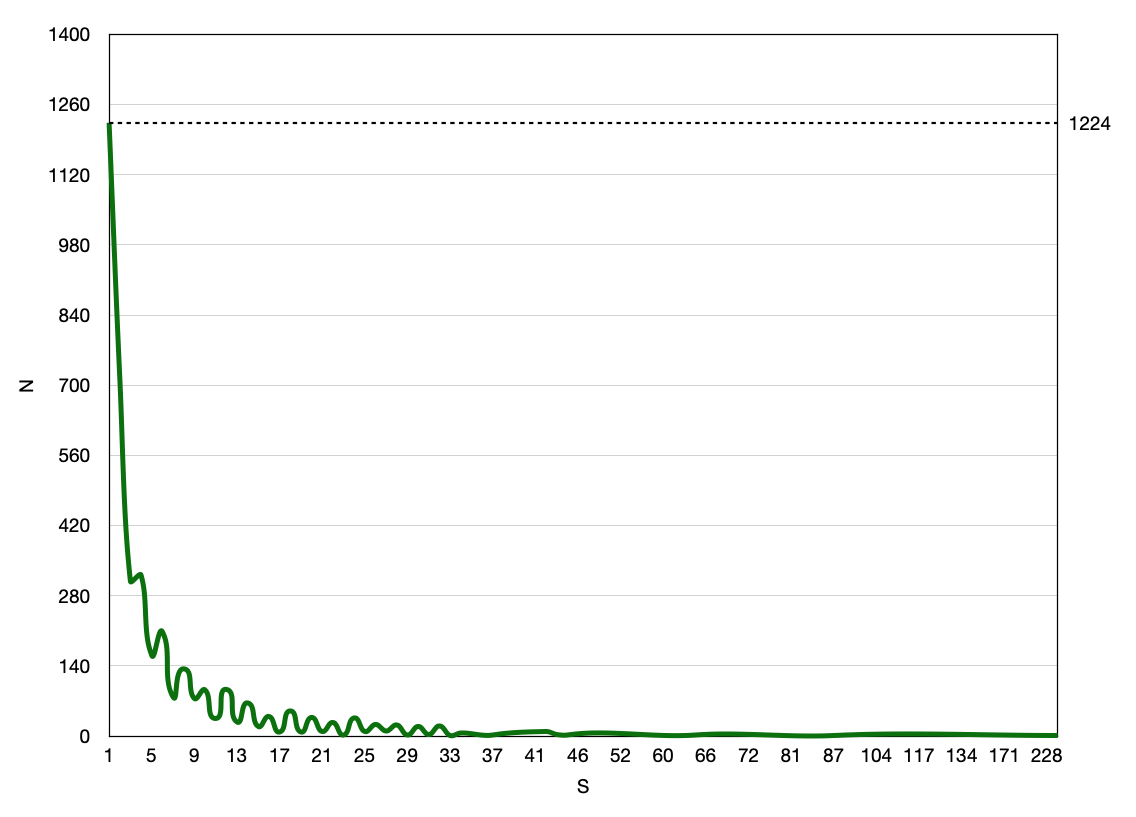
\includegraphics[width=\linewidth]{./chapter/city/Number_of_cities_having_given_number_of_sister_cities_according_to_Wikidata,_2020.png}}
}
  \caption{Зависимость числа городов (N) от числа имеющихся у этих городов побратимов (S), 2020 год.}
  \label{fig:city_relation_S_N}
\end{marginfigure}

Результаты SPARQL-запроса для нахождения числа городов (N) с определенным числом побратимов (S) отображены на рис.~\ref{fig:city_relation_S_N}. Максимальное значение N (1224 города) наблюдается при S, равном единице, затем следует резкое уменьшение числа городов с увеличением числа имеющихся у них побратимов. На рис.~\ref{fig:city_ln_relation_S_N} также представлены полученные данные, но в логарифмической шкале. Так, чуть более четырех тысяч городов (4046 городов) побратались хотя бы с одним городом, из них:
\begin{itemize}
\item 32\% (1314 городов) связаны братскими отношениями более чем с пятью городами;
\item 18\% (728 городов) имеют как минимум одиннадцать городов-побратимов;
\item 9\% (345 городов) подружились более чем с двадцатью городами;
\item 2\% (94 города) имеют от пятидесяти побратимов.
\end{itemize}

\begin{figure*}[h]
{
\setlength{\fboxsep}{0pt}%
\setlength{\fboxrule}{1pt}%
\fcolorbox{gray}{gray}{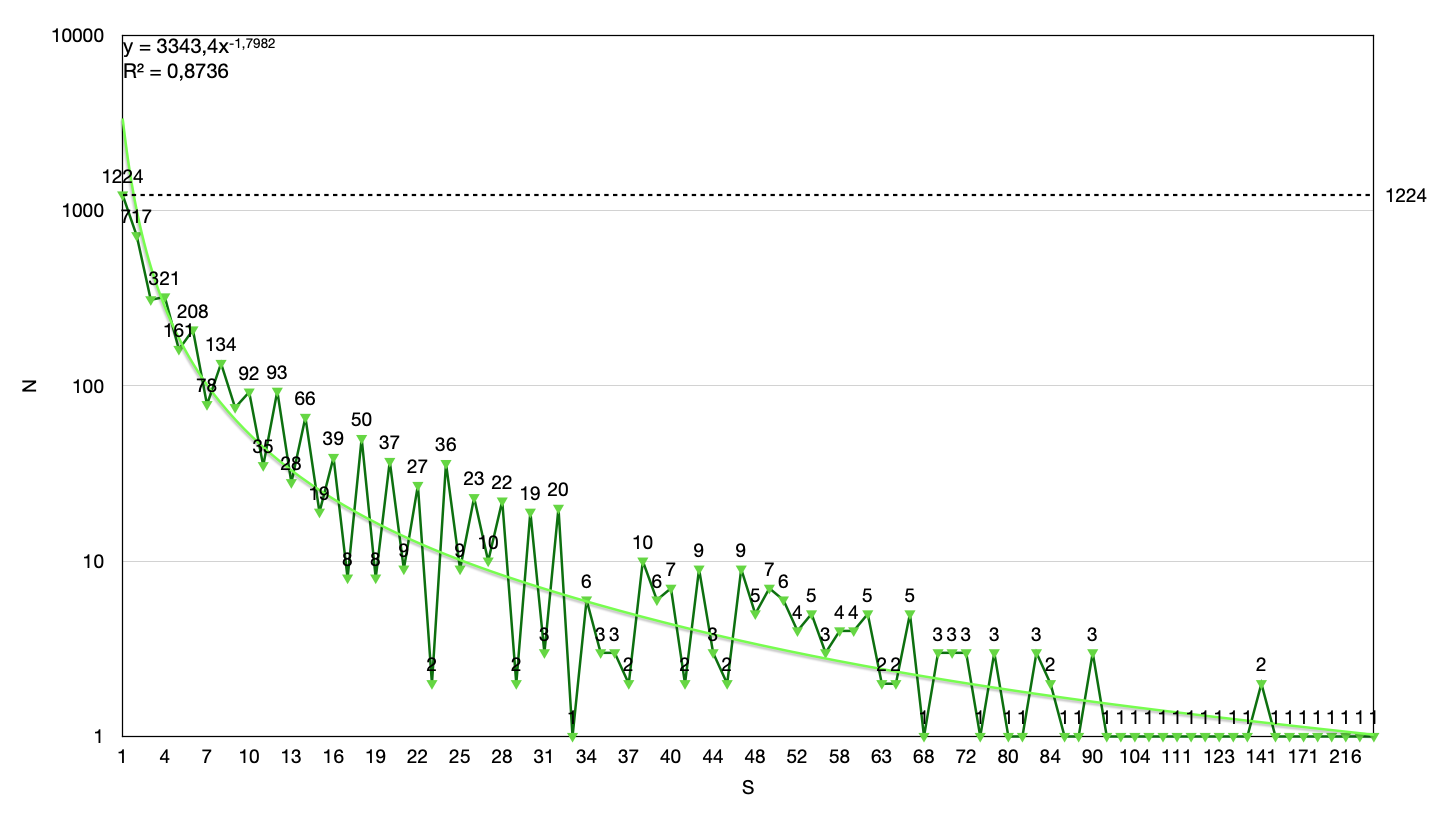
\includegraphics[width=\linewidth]{./chapter/city/Logarithm_of_the_number_of_cities_having_given_number_of_sister_cities_according_to_Wikidata,_2020.png}}%
}
  \caption{Логарифмическая зависимость числа городов (N) от числа имеющихся у этих городов побратимов (S), 2020 год.}%
  \label{fig:city_ln_relation_S_N}%
\end{figure*}

На основании построенного тренда можно сделать предположение, что зависимость числа городов от числа имеющихся у этих городов побратимов имеет распределение, близкое к степенному.